\documentclass{article}
\usepackage[a4paper, total={7.9in, 11.5in}, top=0in, footskip=0.1in, bottom=0.1in, headheight=0.1in, hoffset=0in]{geometry}
\usepackage[utf8]{inputenc}
\usepackage[french]{babel}
\usepackage{graphicx}
\usepackage{graphics}
\usepackage{colortbl}
\usepackage[T1]{fontenc}
\usepackage{amsmath}
\usepackage{hyperref}
\usepackage{array}
\usepackage{amssymb}
\usepackage{colortbl}
\usepackage{color}
\usepackage{listings}
\usepackage{xcolor}
\usepackage{array}
\usepackage{float}
\usepackage{amsfonts}
\usepackage{fancyhdr}
\usepackage{wrapfig}
\usepackage{comment}


\setcounter{topnumber}{2}
\setcounter{bottomnumber}{2}
\setcounter{totalnumber}{4}
\renewcommand{\topfraction}{0.85}
\renewcommand{\bottomfraction}{0.85}
\renewcommand{\textfraction}{0.15}
\renewcommand{\floatpagefraction}{0.8}
\renewcommand{\textfraction}{0.1}
\setlength{\floatsep}{5pt plus 2pt minus 2pt}
\setlength{\textfloatsep}{5pt plus 2pt minus 2pt}
\setlength{\intextsep}{5pt plus 2pt minus 2pt}

\hypersetup{
    colorlinks=true,
    linkcolor=black,
    filecolor=magenta,
    urlcolor=cyan,
    pdftitle={LEPL1252 - Rapport P0 - Matya Aydin Thomas Debelle},
    pdfpagemode=FullScreen,
    }

\title{LEPL1252 - Projet 0}
\author{Matya Aydin \& Thomas Debelle}
\date{Novembre 2023}

\begin{document}

\maketitle

\section{Fonctionnement}


Ajouter les 3 états d'exécution avec un diagramme et mettre les informations de l'algo

\subsection{Structure de la mémoire}

\begin{wrapfigure}{r}{0.4\textwidth}
    \centering
    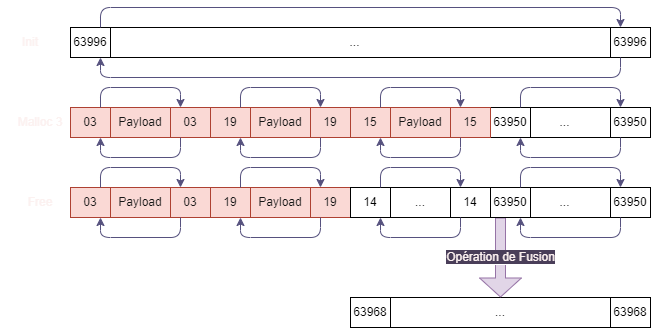
\includegraphics[width=0.4\textwidth, trim={2cm 0 0 0}, clip]{fonctionnement.png}
    \caption{Structure de la mémoire}
    \label{fct}

\end{wrapfigure}

Autour de chaque morceau de mémoire se trouve des informations sur la taille de ce dernier. On y indique le nombre d'octets libres + 1 si le bloc est occupé.
Étant donné que MY\_HEAP est un tableau de 64000 éléments et que nous ne souhaitons pas perdre d'information sur la taille des blocs, nous utilisons 2 bytes pour stocker la taille de ceux-ci.
À la création, on indique donc qu'il y a 63996 octets disponibles. Ce nombre est écrit au début et à la fin de chaque morceau (les avantages de cette structure sont abordés aux sections \ref{free} et \ref{perf}). Ci-dessus, une représentation abstraite de la mémoire.

\subsection{Malloc}
Notre implémentation de `malloc` est la suivante, on met de part et d'autre des cases des données la taille disponible. On alloue que des tailles paires ainsi on peut utiliser le bit de poids faible pour indiquer si les blocs sont libres ou occupés.  Si c'est un nombre pair par exemple 4, il y a donc 4 emplacements libres de chacun 8 bits. Si ce chiffre était 5, cela signifierait qu'il y a 4 octets mais qu'ils ont été alloués par malloc.\\ 
En cas de demande d'un nombre impair, la taille du bloc retourné est augmentée de 1.\\
On commence par chercher le premier ensemble de blocs qui puissent accueillir la taille désirée par l'utilisateur. On commence au début de notre Heap à chaque fois.\\
2 critères d'arrêt sont considérés:
\begin{itemize}
    \item la fin de MY\_HEAP est atteinte sans avoir trouvé un emplacement non-alloué suffisamment grand: la recherche s'arrête et NULL est renvoyé à l'utilisateur.
    \item Un bloc libre de taille supérieure ou égale à la taille demandée est trouvé: la recherche s'arrête. \newline
\end{itemize}

Si la taille du bloc trouvé est supérieure à la taille demandée, malloc va partitionner en 2 morceaux notre mémoire. Seul le premier est allouée et la fonction malloc s'occupe directement d'indiquer que la suite du bloc est toujours libre.

%On va donc partitionner un ensemble de blocs en 2 plus petits ensembles. Le premier des deux a la taille désirée par l'utilisateur et le deuxième est le reste des blocs.\\ 
Il est important de noter qu'à chaque fragmentation de notre mémoire, 4 octets (2 à chaque nouvelle extrémité représentant la taille du bloc) de méta-données sont requis.

\subsection{Free}
\label{free}
Notre free va éviter la fragmentation de la mémoire. En effet, on regarde si les fragments de mémoire à droite et à gauche de celui qu'on veut libérer sont libres.
Cela est permis en $\mathcal{O}(1)$ grâce au fait que chaque bloc a directement accès aux tailles (et à l'état) du bloc précédent et du bloc suivant grâce aux méta-données présentes aux 2 extrémités.
Si c'est le cas on va regrouper nos fragments en un seul comme montré à la figure \ref{fct}.\\
Nous ne remettons pas les octets fraîchement libérés à 0 pour éviter une consommation de ressources inutiles. Leurs valeurs seront simplement écrasées lorsque la zone mémoire sera à nouveau allouée et que l'utilisateur écrira par dessus. On ne fait rien si l'utilisateur essaye de libérer des octets déjà libres et un message le stipulant est affiché.

\section{Discussion \& Performances}
\label{perf}

\subsubsection*{Motivation du choix d'algorithme}
%Notre politique first fit a pour avantage d'être rapide. Cependant, elle ne rime pas avec localité. En effet, on ne garantit pas que des valeurs associés à la chaine (donc des valeurs qui risquent d'être accédées à la chaine) sont l'une à côté des autres.\\
%Tout du moins, on évite la fragmentation via notre implémentation de free qui va regrouper les blocs inutilisés.
Malgré un malloc en $\mathcal{O}(N)$ et 4 bytes de méta-données nécessaires par blocs, notre implémentation favorise la localité temporelle.\\
Commencer chaque recherche au début du tableau permet de n'ignorer aucun bloc potentiellement libéré durant l'exécution du programme.\\
2 autres aspects de notre implémentation minimise également la fragmentation:
\begin{itemize}
    \item Malloc n'alloue que la taille nécessaire et séquence directement un bloc de taille supérieure et un bloc alloué de la taille demandée suivi d'un bloc libre de la taille restante 
    \item Un free ayant accès au bloc précédent et au bloc suivant afin de les fusionner si nécessaire\newline
\end{itemize}

Un autre défaut mineur de notre implémentation est la possibilité de n'allouer que des blocs de taille paire.
\end{document}